\subsection*{Интуиция и идея kNN}

\begin{example}
Рассмотрим картинку. Путь у нас все объекты двух типов -- синий квадрат или красный треугольник. И вот нам поступил объект, который на картинке отмечен зеленым кружочком. Мы про него хотим понять, кто он на самом деле (к какому из двух классов относится). Это несложно делается с помощью метода ближайших соседей.
\end{example}

\begin{center}
    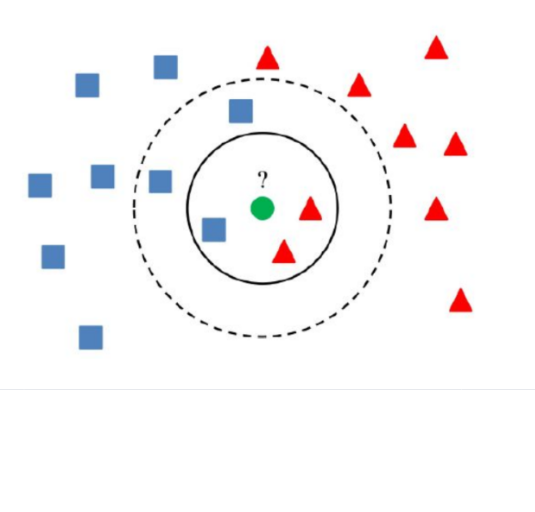
\includegraphics[scale=0.7]{images/6_1.png}
\end{center}

Собственно, плюс метода ближайших соседей как раз в том, что он абсолютно интуитивный. Идея такая: <<чем ближе я к другим объектам в признаковом пространстве, тем больше я на них похож>>. 
Мы можем использовать расстояние между объектами в пространстве признаков как некоторую меру похожести.

Допустим на картинке мы будем считать расстояние по $L2$-норме, то есть использовать Евклидово расстояние, к которому мы привыкли. В этой и других задачах в прицнипе можно ввести любую другую метрику и по ней посчитать расстояние.

Если у нас просто есть выборка, и она желательно задана в каком-то линейном метрическом пространстве, то, как правило, там мало категориальных фичей, этим можно воспользоваться и применить собсвенно описанную выше идею. Вот тут появляется выбор гиперпараметра модели: тут это параметр $k$ -- сколько ближайших соседей мы выбираем для того, чтобы решить, к какому классу относится объект. Если мы возьмем одного соседа, он может оказаться выбросом из выборки и дать нам неверный результат. Но если мы возьмем информацию о нескольких соседях, мы будем более уверены в предсказании класса объекта. 

\begin{example}[Пример из жизни, поясняющий интуицию:]
Так, например, если вокруг вас вечером много физтехов, то вы, скорее всего, студент физтеха и находитесь в общежитии. 
\end{example}

\subsection*{Алгоритм kNN}

В итоге получаем такой алгоритм:

\begin{enumerate}
    \item Берем датасет и запоминаем координаты объектов в пространстве признаков.
    \item Берем новое наблюдение и считаем все расстояния до каждого объекта в датасете.
    \item Выберем $k$ объектов с минимальным расстоянием до вашего нового наблюдения.
    \item Выбираем класс, который доминирует среди этих $k$ соседей. Он-то и будет нашим предсказанием для рассматриваемого объекта.
\end{enumerate}

Есть минусы в таком подходе:

\begin{enumerate}
    \item При разных значениях гиперпараметра числа соседей может получаться различный результат. Можем проверять качество работы алгоритма при фиксированном параметре, но не можем сходу оптимизировать его (оптимизируется только перебором, к сожалению).
    \item В настоящее время при больших выборках занимает большое вычислительное время из-за подсчета большого количества расстояний (а в пространствах с большой размерностью расстояния считаются между длинными векторами, что тоже долго, все ведь помним плюсы с длинной арифметикой :) ).
\end{enumerate}


\subsection*{Взвешенный kNN}

Теперь подумаем, как еще мы можем предсказывать класс на основе информации о $k$ ближайших сосседях. Сейчас мы выбираем самый часто встречающийся класс, но, может быть, можно делать лучше? Есть такой выход.

Он называется взвешенным $kNN$. В этой вариации мы  присваиваем вес лейблу каждого соседа в зависимости от расстояния от нашего объекта до соседа. То есть чем дальше сосед, тем меньший вклад в ответ он вносит.

\subsection*{Как с помощью $kNN$ решить задачу регрессии?}

Практически ничего не меняется, только таргетами станет континуальная величина, то есть числа.
Что надо сделать с матрицей признаков перед тем как использовать на ней $kNN$?

Ее обязательно надо отнормировать. 

\begin{example} Если в одной матрице есть признак в сантиметрах и признак в метрах, то это странно. Или в бухгалтерии зарплата представлена в матрице в рублях и в копейках как два разных признака, то 
по-хорошему их надо объединить в один признак или привести в одну шкалу, то есть чтобы были рубли и доли рублей. 
\end{example}

Если мы ничего не знаем о природе нашей выборки, то самое лучшее, что мы можем с ней сделать, это отнормировать ее в промежуток $[0;1]$, то есть вычесть минимум и поделить на максимум.